\section{Scalability} \label{sec:scalability}
    The following section describes how Tagion achieves scalability. A Hashgraph allows the system to add information quickly and with minimal communication. To read data, Tagion utilises the deterministic \gls{finality} of the Hashgraph to make the system stateless. To do this efficiently Tagion uses the \gls{dart}.

\subsection{Writing Information}
    As mentioned in the previous chapter, the Hashgraph sends close to the minimum amount of information necessary. This reduces the possibility of communication bandwidth becoming the bottleneck of the system. This, in combination with the Hashgraph consisting of a fixed number of nodes, allows both consensus and ordering to happen with great speed - much greater than in any decentralised blockchain. In total, it is fast to \textit{write} data into the system.

\subsection{Reading Information}
    A system which reaches agreement fast does little good if it cannot communicate what it has agreed upon effectively. We discuss the limits of blockchain systems and how the Hashgraph overcomes these by using the \gls{dart} and deterministic \gls{finality}.

\subsubsection{The Problem with Blockchain Systems}
    For blockchains to be fast, forking must happen often, resulting in one not being able to blindly trust the newest broadcasted block. A node wanting to read the state of the system must continually decide which blocks to trust and which to disregard, so significant effort is required to read the system's current state. Probabilistic \gls{finality} is at the heart of this problem: A blockchain never becomes fully confident that a state will be accepted in the network, only more and more confident with time. Either new states are broadcasted often enough that there is doubt about the validity of the state (forking), or rarely enough that it limits the system's speed. The FLP-theorem\cite{flp_impossibility} proves that no \gls{abft} system can achieve \textit{\gls{liveness}} and \gls{finality}; said differently, no \gls{abft} system can \textit{ensure progress} while simultaneously achieving \gls{finality} (a guarantee that progress will not be overridden). Thus, blockchains cannot achieve \gls{finality} - it is mathematically impossible. This lack of \gls{finality} limits the system's scalability.

\subsubsection{The Hashgraph's Solution - Finality}
    The Hashgraph as a consensus protocol prioritises \gls{finality} above \gls{liveness}. Initially, it might sound problematic that Tagion cannot be sure of progress, but it can, in fact, be certain that progress eventually happens with a 100\% probability. Instead of being certain of progress and probabilistically sure it will not be changed (like blockchains), Tagion is probabilistically sure of progress and certain it will not be changed. Having \gls{finality} comes with significant benefits:

\subsubsection{Using Finality to Achieve Read-scalability}
    Having \gls{finality} in the Tagion system allows for scalability in a way not possible in systems without it. When nodes in the Tagion network agree on a new state of the system, they push it to all listeners along with a signature from all nodes. Due to \gls{finality}, all nodes can trust the broadcasted state just by verifying the signature. This makes the system stateless, meaning that any node only needs to remember the current state of the system. This is in contrast to blockchain systems where the history of states defines the consensus; making it a necessity to store the history of the system. This increases hardware requirements to participate in the system, resulting in centralisation as a side effect. Since Tagion is stateless, it avoids these problems. It is thus easy to read the state of the system \textit{if} we have an efficient and effective way to continuously verify the broadcasted signed states. To do this Tagion uses the \gls{dart}, a database which retains the byzantine proof from the consensus layer.

\subsection{DART}
    The \gls{dart} is how Tagion stores the data in the network. The \gls{dart} handles removal and addition of data, and computing \textit{the bullseye} to represent a signature of the system. The main problem the \gls{dart} solves, is fast recomputation of the bullseye after some parts of the database changes. 

\subsubsection{Structure}
    The \gls{dart} is a database storing archives, a flexible data structure that can hold different types of files. At its core, the \gls{dart} is a Distributed Hash Table (DHT), which means that archives are stored based on its hash-key. The hash of an archive thus determines where the archive is stored. The database can be represented as a circular structure: A dart-board with branches of data growing from the center. The more archives that are stored in the system, the more branches the \gls{dart} creates. The following describes the \gls{dart} through the proceeding example\footnote{For explanatory purposes, the example shows the \gls{dart} with rim 1, 2, and 3. In practise, the first 2 rims are kept clear of archives and store only branches, and the \gls{dart} also contains many more rims. The shown hashes are also 6 hexadecimals long, where as real hashes are 64 hexadecimals long.}.

    \pagebreak
    
\begin{figure}[H]
 \centering
 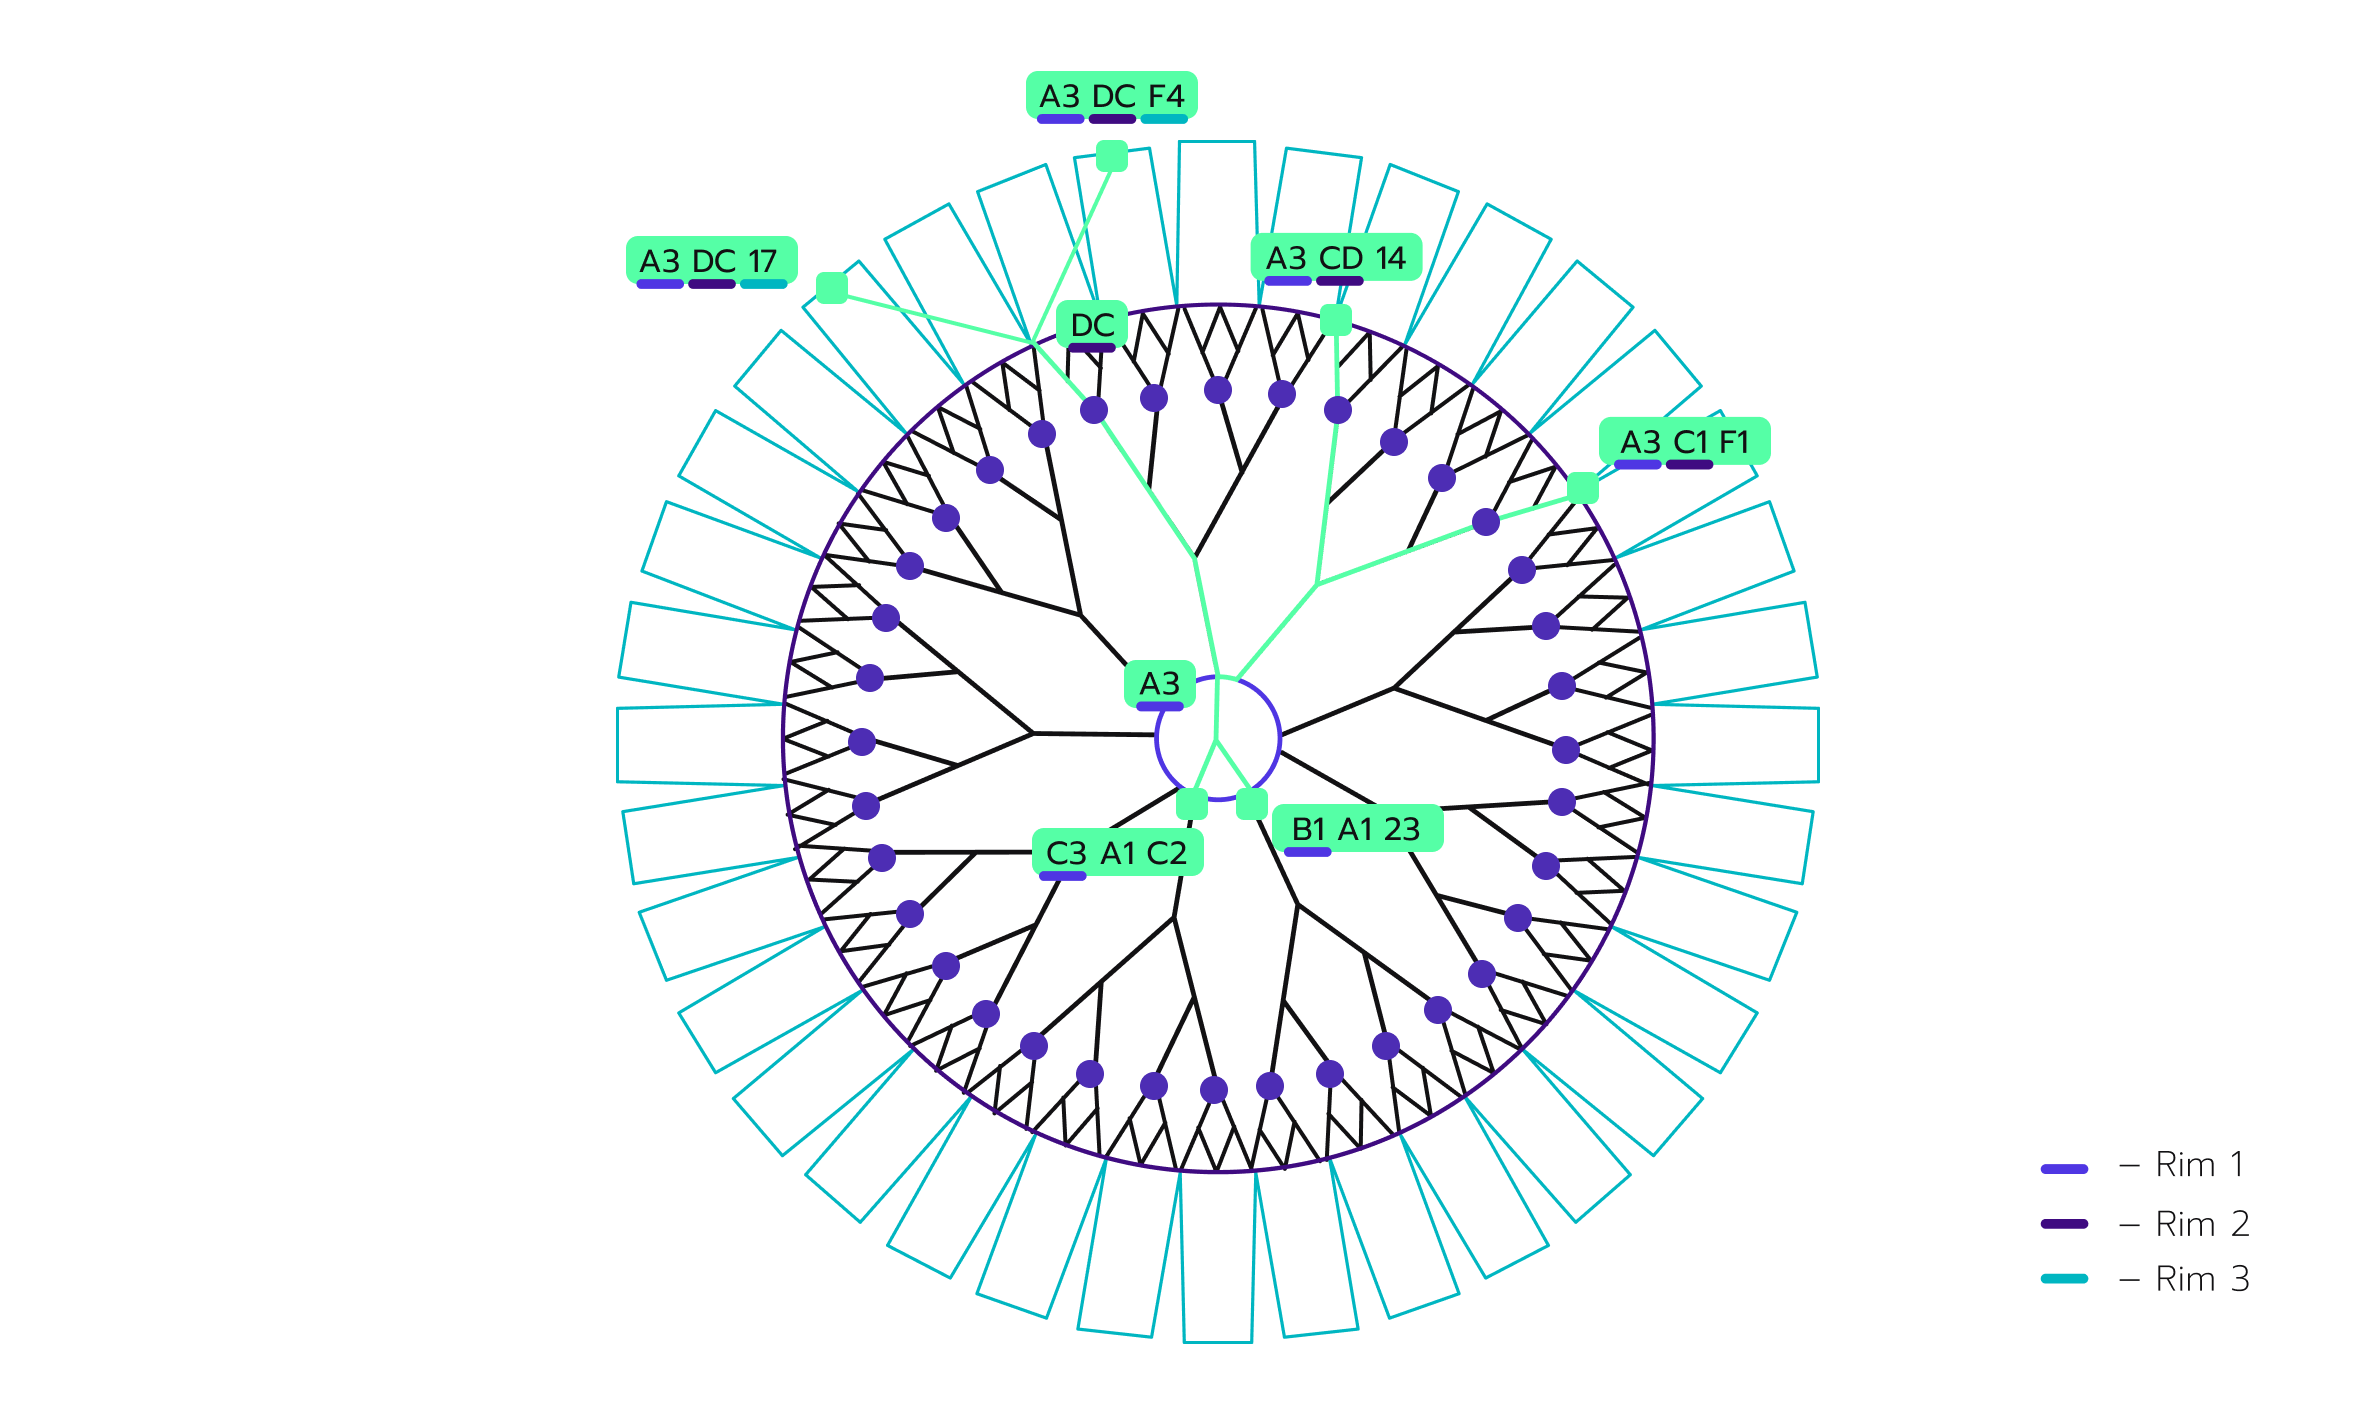
\includegraphics[width=1 \textwidth]{figures/dart_structure.png}
 \caption{The structure of the DART database}
 \label{fig:dart_structure}
\end{figure}

    The \gls{dart} consists of multiple rims, the number of rims increasing with the total number of archives. The first 2 hexadecimals of the archive's hash determines where in rim 1 it is stored. If the first 2 hexadecimals are unique (e.g. C3 or B1 on the figure) this archive is stored at rim 1. On the other hand, if multiple archives share the first 2 hexadecimals of their hash (e.g. A3), then the dart creates a branch at A3 and stores this data on the next rim (e.g. A3-CD-14 and A3-C1-51). If multiple archives \textit{also} share the third and fourth hexadecimal we create a further branch (e.g. DC). Each branch has at most 256 combined archives and subbranches. The \gls{dart} adds and removes data in a way that ensures that the \gls{dart} always has the minimum number of branches and rims. The more rims in the \gls{dart} the more compute it takes to retrieve data, so it is essential to keep the number of rims minimal. The DART can maximally store 32 rims; using just 29 of these it could store every atom in the Milky Way in individual archives. So, storage capacity of the \gls{dart} will never become a problem. Tagion also uses the \gls{dart} to generate \gls{udr} data, used to agree on truly random choices.

\subsubsection{State of the System}
    The reason for using this structure is that it makes recomputing the signature of the system, the \gls{bullseye}, very efficient. The \gls{dart} can be viewed as a \gls{smt}. Each branch computes its hash based on all the hashes of its subbranches/archives (of which there are up to 256). To compute the \gls{bullseye}, one needs to compute the hashes from the outermost rim and compute hashes inwards until one reaches the innermost rim: The \gls{bullseye}. In the provided example one would first compute the hash of the archives in rim 3. Then we would compute the hash of the archives in rim 2, where the hash of branch DC is computed by combining the hash of A3 DC 17 and A3 DC 54. Finally it computes the hash of archives in rim 1 (where the hash of branch A3 is based on the hashes of branch DC, archive A3 CD 14, and archive A3 C1 F1), and then combines these to the \gls{bullseye}. During the computation of the \gls{bullseye}, one saves the calculated hashes. This is the \textit{crucial} step which allows the \gls{dart} to recomputate the \gls{bullseye} quickly. When the \gls{dart} changes and one needs to compute a new \gls{bullseye}, it is only necessary to recompute the hashes of the branches which changed, which will be a tiny fraction of the system in practise. For example, consider if only the archive B1-A1-23 changes. Computing the \gls{bullseye} only requires hashing this single archive and combining rim 1 to get the \gls{bullseye}, since all other hashes are saved from the last \gls{bullseye} calculation. In this way one can continuously, efficiently calculate the \gls{bullseye}: A signature of the entire system.

\subsection{A Stateless Scalable System}
    Once consensus is reached in the Tagion system, nodes broadcast the state and its signed \gls{bullseye}. Passive nodes, or any individual wanting to know the state of the system, can subscribe to these broadcasts. Using the \gls{dart}, receivers can verify the \gls{bullseye} quickly, with minimal computation. This results in a stateless system where we don't need to save previous states of the system. This allows for deletion of data (as we don't need to store data from a previous state) and results in storing less data overall. Not only does this make the system scalable, it also decreases the hardware requirements for participating in the network. Thus, the barrier to participate in the system is lower, increasing the degree of decentralisation. It is important to note that our system is open to the possibility of storing past states. This might be important for some actors who want to use the full history. In practise few nodes would store the entire history, while most nodes would only maintain the current state. In blockchain systems one is forced to save the history; in the Tagion system one has the \textit{option} of saving it \textit{only} if deemed necessary. In the next section we discuss how Tagion utilises \textit{swapping} to achieve a fully decentralised system.
\pagebreak